\chapter{Estructura del proyecto subido a GitHub}

El código fuente de todo el proyecto está subido en un repositorio público en GitHub y es accesible para poder realizar las mismas pruebas desarrolladas en este \gls{tfg}.

El proyecto entero se puede encontrar en \href{https://github.com/ems107/EdgarMartinezSerranoTFG}{GitHub} desde el siguiente enlace:

\href{https://github.com/ems107/EdgarMartinezSerranoTFG}{https://github.com/ems107/EdgarMartinezSerranoTFG}.

Dentro de la estructura del proyecto, nos encontraremos con un README que nos explicará cómo compilar y ejecutar del proyecto.

\begin{figure}[h]
    \centering
    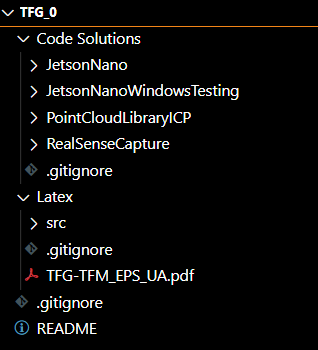
\includegraphics[height=6cm]{archivos/estructura-proyecto.png}
    \caption{Estructura del proyecto en GitHub.}
    \label{fig:estructura-proyecto}
\end{figure}

En la Figura \ref{fig:estructura-proyecto} podemos ver cómo se estructura el repositorio.
Por un lado tenemos el directorio ``Latex'' donde podemos encontrar todo el código fuente utilizado para construir esta memoria, y la memoria en sí.

Por otro lado, dentro del directorio ``Code Solutions'' encontraremos todo el código utilizado en el \gls{tfg}.
Dentro del subdirectorio ``JetsonNano'' encontramos el proyecto CMake que se ha estado explicando detalladamente en la memoria.
En el subdirectorio ``JetsonNanoWindowsTesting'' encontramos una solución en Visual Studio capaz de ejecutar el mismo código que ha sido desarrollado en la Jetson para testear en Windows, excluyendo la librería de CUDA-ICP que no funciona en Windows.
Por último, los subdirectorios ``PointCloudLibraryICP'' y ``RealSenseCapture'' son pequeñas soluciones en Visual Studio con diversas pruebas sobre estas librerías.